\documentclass[svgnames]{amsart}
\usepackage[paperwidth=6in, paperheight=8in, top = 20mm, bottom = 18mm, left=10mm, right = 10mm]{geometry}

\usepackage{amsmath, amsfonts, amssymb, amsthm}
\usepackage{graphicx, tikz}
\usepackage{mathtools, physics}

\usepackage{enumitem}
\setlist[enumerate,1]{label=\arabic*.}

\usepackage[default,bold]{sourceserifpro}
\usepackage[T1]{fontenc}
\usepackage{eulervm}

\usepackage{xcolor}

\renewcommand{\th}{\textsuperscript{th}}

\setlength{\parindent}{0pt}

\title[]{Probability and Statistics -- Problem Set 6}

\DeclareMathOperator{\Prob}{P}
\DeclareMathOperator{\EV}{\mathbb E}
\DeclareMathOperator{\Var}{\mathbb V}


\begin{document}
\maketitle
\begin{enumerate}[leftmargin=*]
\item If $Z \sim N(0,1)$, compute
\begin{enumerate}
	\item $\Prob[Z < 1]$
	\item $\Prob[Z < 2.4]$
	\item $\Prob[1 < Z < 2.4]$
	\item $\Prob[Z < -1]$
	\item $\Prob[-2.4 < Z < 1]$.
	\item $\Prob[|Z| > 1]$
\end{enumerate}

\item If $X \sim N(175, 25^2)$, compute
\begin{enumerate}
	\item $\Prob[X < 200]$
	\item $\Prob[X < 235]$
	\item $\Prob[200 < X < 235]$
	\item $\Prob[X < 150]$
	\item $\Prob[115 < X < 200]$.
\end{enumerate}

\item In a normal distribution, $31\%$ of the observations are under $45$ and $8\%$ are over $64$. Find the mean and standard deviation.

\item In a normal distribution, $7\%$ of the observations are under $35$ and $89\%$ are under $63$. Find the mean and standard deviation.

\item Suppose that the life lengths of two electronic devices $D_1$ and $D_2$ (in hours) have distributions $N(40, 36)$ and $N(45, 9)$ respectively. If the device is to be used for a $48$ hour period, which device is to be preferred?

\item Suppose that the scores of an examination are normally distributed with mean $76$ and standard deviation $15$. The top $15\%$ scores receive grade A and the bottom $10\%$ receive grade F. Find
\begin{enumerate}
	\item the minimum score to receive an A
	\item the minimum score to pass.
\end{enumerate}

\item Suppose that the heights of $800$ students are normally distributed with mean $66''$ and standard deviation $5''$. Find the number of students with heights
\begin{enumerate}
	\item between $65''$ and $70''$
	\item greater than or equal to $6'$.
\end{enumerate}

\item In a certain examination, the percentages of candidates passing and getting distinction were $45$ and $9$ respectively. Assuming that the marks are normally distributed, determine the average marks obtained by a candidate if the minimum marks for passing and distinction are $40$ and $75$ respectively.
\end{enumerate}

\includegraphics[trim = 65 30 50 95, clip, page=2, width=\linewidth]{Statistical Tables.pdf}

\end{document}